	% 代码分析:模块功能、涉及到的类、类关系、数据结构及关键代码等;
	% 任务要求,设计任务要求;
	% 设计:详细的设计方案,相关的数据结构、算法描述,可采用伪代码等形式化描述
	% 实现:修改哪些类、如何修改、为什么修改等;
	% 测试:测试用例,测试结果及结果分析,测试运行界面等;
	% 调试:调试方法,遇到的问题及解决方案等;
	% 结论与展望:完成的主要工作、收获、进一步的工作,建议、体会、心得等;

\section{作业9}
\subsection{题目描述}
\begin{figure}[H]
    \centering
    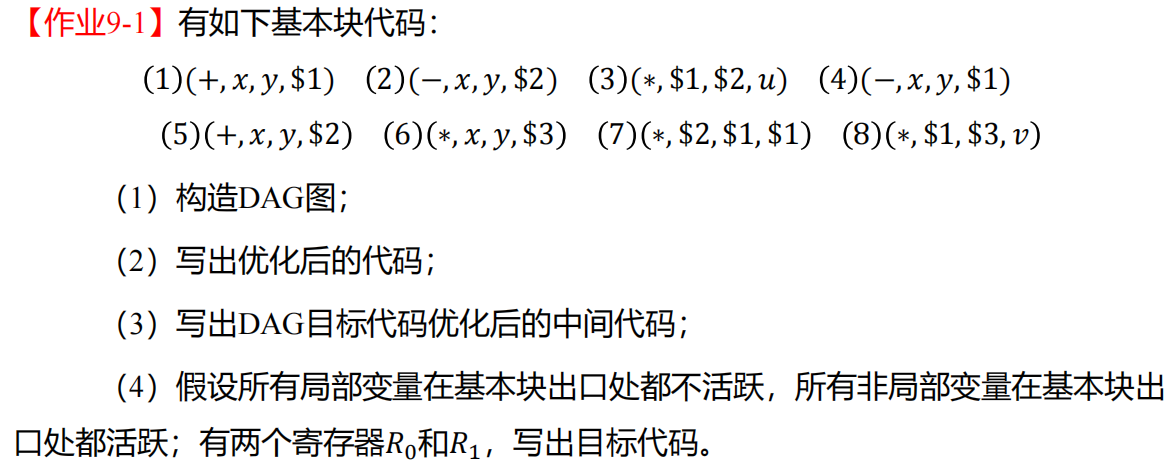
\includegraphics[width=0.9\linewidth]{imgs/9_1.png}
    \caption{作业 9.1——题目}
    \label{fig:9_1_prob}
\end{figure}
\subsection{解答}
\paragraph{构造 DAG 图、写出优化后的代码} 注意到两次计算 $x+y$ 与 $x-y$,分别赋给 \$1、 \$2 与 \$2、 \$1,可以重排 DAG 节点,同时不难对照 DAG 图写出代码:


\begin{table}[H]
    \centering
    \begin{tabular}{cc}
    \centering
    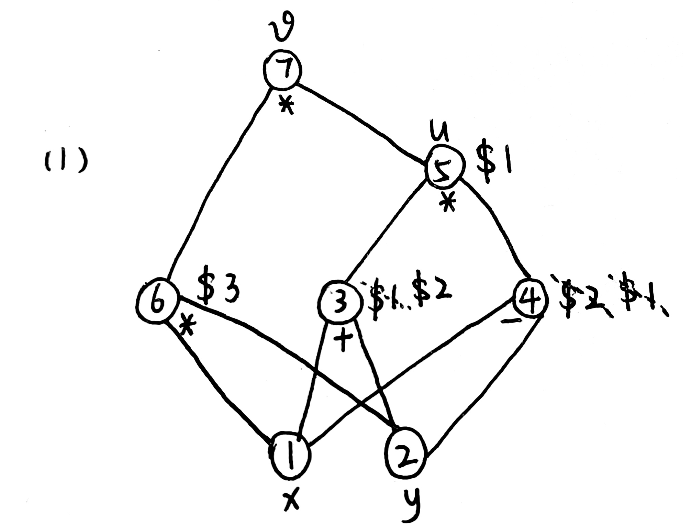
\includegraphics[width=0.4\linewidth]{imgs/9_1_1.png}
    & 
\begin{tabular}{rl}
(1) & $(+, x, y, \$1)$ \\
(2) & $(-, x, y, \$2)$ \\
(3) & $(*, \$1, \$2, u)$ \\
(4) & $(*, x, y, \$3)$ \\
(5) & $(*, u, \$3, v)$
\end{tabular}
\\
    \end{tabular}
\end{table}

\paragraph{写出 DAG 目标代码优化后的中间代码} 可以写出:

\begin{tabular}{rl}
(1) & $(*, x, y, \$3)$ \\
(2) & $(+, x, y, \$2)$ \\
(3) & $(-, x, y, \$\$1)$ \\
(4) & $(*, \$2, \$\$1, u)$ \\
(5) & $(*, \$3, u, v)$
\end{tabular}

\paragraph{写出目标代码} 可以写出:

\begin{table}[H]
\begin{tabular}{rll}
(1) &\quad$(*, x, y, \$3)$& \quad \text{\texttt{MOV R0 [ebp-$\hat \delta_x$]}} \\
  && \quad \text{\texttt{IMUL R0 [ebp-$\hat \delta_y$]}} \\
(2) &\quad$(+, x, y, \$2)$& \quad \text{\texttt{MOV R1 [ebp-$\hat \delta_x$]}} \\
  && \quad \text{\texttt{ADD R1 [ebp-$\hat \delta_y$]}} \\
(3) &\quad$(-, x, y, \$\$1)$& \quad \text{\texttt{MOV [ebp-$\hat \delta_{\$3}$] R0}} \\
  && \quad \text{\texttt{MOV R0 [ebp-$\hat \delta_{x}$]}} \\
  && \quad \text{\texttt{SUB R0 [ebp-$\hat \delta_{y}$]}} \\
(4) &\quad$(*, \$2, \$\$1, u)$& \quad \text{\texttt{IMUL R0 R1}} \\
(5) &\quad$(*, \$3, u, v)$& \quad \text{\texttt{MOV [ebp-$\hat \delta_{\$3}$] R1}} \\
  && \quad \text{\texttt{MOV [ebp-$\hat \delta_{u}$] R1}} \\
  && \quad \text{\texttt{IMUL R0 R1}} \\
  && \quad \text{\texttt{MOV [ebp-$\hat \delta_{v}$] R0}}
\end{tabular}
\end{table}
